En los ejemplos anteriores se ha evaluado la precisión del método de Taylor con y sin el Transporte de Jets. Hemos estudiado casos hamiltonianos en donde las soluciones a las ecuaciones diferenciales viven en curvas de energía constante sobre el espacio fase. Es importante tener en cuenta que éste es sólo un subconjunto de casos en la familia de sistemas de ecuaciones diferenciales ordinarias. Nuevos elementos aparecen en los campos vectoriales impuestos por la forma más general de (\ref{eq:ode}) como órbitas periódicas, atractores, repulsores o atractores extraños \cite{Perez2015}. La idea de los indicadores dinámicos radica en encontrar estructuras que nos permitan catalogar a los campos vectoriales, sean hamiltonianos o no, y sacar información relevante acerca de las soluciones al sistema de ecuaciones dado. 

Hay que destacar que el Transporte de Jets no sirve únicamente para dar indicadores dinámicos del espacio fase. Hay un montón de cosas que se pueden aprovechar al tener la solución parametrizada por polinomios. Entre éstas están hacer simulaciones de Montecarlo o hacer variación de los parámetros de las ecuaciones.

\subsection{Un poco de motivación vía exponentes de Lyapunov}
\label{sec:FTLE}

El Transporte de Jets nos permite saber qué pasa con el flujo entre condiciones iniciales vecinas. En este sentido, si se hace un transporte alrededor de $\xo$, sabemos como es el flujo de $\xo + \delta \xo$. Por esto, los Exponentes de Liapunov a Tiempo Finito (ELTF) emergen commo una motivación natural a los indicadores que serán propuestos en este capítulo. Un ELTF es, sin entrar en muchos detalles, el promedio en un lapso finito de tiempo de la tasa de máxima expansión entre dos condiciones iniciales cercanas. La construcción que aquí se plantea sigue a Shadden, Lekien y Marsden en \cite{Shadden2005}.

Consideremos dos condiciones iniciales vecinas $\xo$ y $\mathbf{\chi}_0 = \xo + \delta \xo$ en $\mathcal{D} \subset R^d$ con flujos $\phi(T;t_0, \xo)$ y $\phi(T;t_0, \chi_0)$, respectivamente, después de un intervalo $T$ de tiempo, con $\delta \xo \ll 1$ y en alguna dirección arbitraria . La diferencia después del intervalo $T$ es

\begin{equation}
 \delta \mathbf{x}(T) = \phi(T;t_0, \chi_0) - \phi(T;t_0, \xo) = \frac{d \phi(T;t_0, \xo)}{d\xo} \delta \xo + \mathcal{O} \left( \norm{ \delta \xo}_2^2 \right).
 \label{eq:perturbation}
\end{equation}

Ignorando el término de orden cuadrático en $\delta \xo$, se puede encontrar la magnitud de la perturbación al tiempo $T$ via la norma estándar

\begin{equation}
 \norm{\delta \mathbf{x}(T)}_2 = \sqrt{ \left\langle \frac{d \phi(T;t_0, \xo)}{d\xo} \delta \xo, \frac{d \phi(T;t_0, \xo)}{d\xo} \delta \xo \right\rangle }.
 \label{eq:perturbation_norm}
\end{equation}

La máxima expansión de (\ref{eq:perturbation_norm}), se encuentra en la dirección donde $\delta \xo$ esté alineada con el eigenvector asociado al máximo eigenvalor de la matriz\footnote{Esta matriz se suele conocer como el tensor (derecho) de Cauchy-Green.}
\begin{equation}
 \Lambda(\xo, T) := \frac{d \phi(T;t_0, \xo)}{d\xo}^* \frac{d \phi(T;t_0, \xo)}{d\xo}.
 \label{eq:finite_cgtensor} 
\end{equation}
Es decir, 
\begin{equation*}
 \max_{\delta \xo} \norm{\delta \mathbf{x}(T) } = \sqrt{ \lambda_{max}(\Lambda) \norm{ \delta \tilde{\xo}}^2 } = e^{\sigma(\xo,T)\lvert T \rvert} \norm{ \delta \tilde{\xo} }  ,
\end{equation*}
con $ \delta \tilde{\xo} $ en la dirección del eigenvector asociado a $\lambda_{max}(\Lambda)$ y
\begin{equation}
 \sigma(\xo,T) := \frac{1}{2 \lvert T \rvert} \ln \lambda_{max}(\Lambda(\xo, T)),
 \label{eq:FTLE}
\end{equation}
el máximo ELTF integrado a tiempo $T$ asociado al punto que en $t_0$ pasa por $\xo$. Como se mencionaba al principio de la sección, $\sigma(\xo,T)$ nos da la tasa de máxima expansión de $\xo$ promediada en el intervalo $T$. Calcular el ELTF es fácil con el TJ ya que, por la parametrización polinomial de $\flowxi$, $\lambda(\xo,T)$ se puede calcular directamente usando jets de orden $M = 1$. Con esto, se puede estudiar el espacio fase de una campo vectorial dado ya que diferentes valores de $\sigma$ representan diferentes tasas de expansión para la misma escala temporal.

%FIGURA!
\begin{figure}[h!]
 \centering
 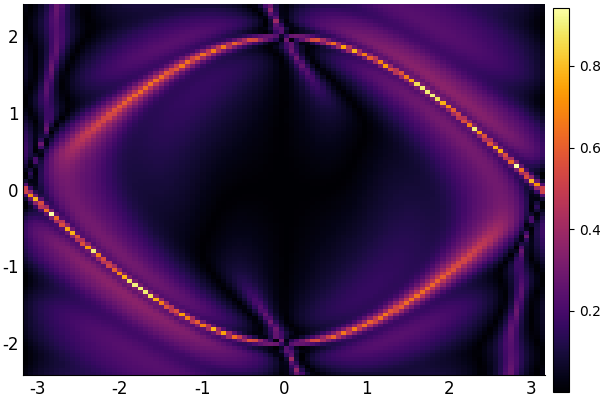
\includegraphics[width=0.7\linewidth]{ftle_pendulum}
 \caption{Campo escalar de los ELTF calculada con (\ref{eq:FTLE}) para el péndulo de (\ref{eq:pendulo-ode}) en una retícula de $100$ puntos por lado, después de un periodo, con tolerancia $\epsilon_{Taylor} = 10^{-10}$ y orden máximo de la expansión $M = 25$.}
 \label{fig:ftle_pendulum}
\end{figure}

La figura \ref{fig:ftle_pendulum} presenta al campo escalar de los ELTF calculados a partir de (\ref{eq:FTLE}) para el péndulo simple descrito por (\ref{eq:pendulo-ode}). Es interesante cómo la separatrices del péndulo coinciden con los valores más grandes de $\sigma$ en el espacio fase. En \cite{Haller2011}, se hace un análisis profundo para detectar diferentes regiones en el espacio fase, que ahí nombra como Estructuras Lagrangianas Coherentes, motivado en la parcelas lagrangianas de la mecánica de fluidos. Como se muestra en la referencia anterior, no necesariamente el campo escalar de ELTF va a encontrar separatrices, sino puntos cuyas soluciones vecinas se alejan rápidamente en el tiempo; esto puede indicar, sí, separatrices, pero también caos, o grandes gradientes de velocidad en el espacio fase.

%Casos donde esto falla o donde el jacobiano no es suficientemente buena aproximación... 

\pagebreak
\subsection{Tamaño máximo de las vecindades}
\label{sec:ximax}

Los ELTF son una buena herramienta para ver la tasa de expansión de la variacion entre dos condiciones vecinas. Esto es una buena motivante para el Transporte de Jets, ya que no se tiene, a priori, la restricción de la linealidad que se tiene en el caso anterior. Lo único que se hizo para adaptar el TJ al campo de ELTF fue tomar un desarrollo a primer orden de las soluciones de un campo vectorial dado. Sin embargo, si las expansiones de los polinomios son de orden $N > 1$, entonces las deformaciones en las vecindades de $\xo$ exhibirán términos no lineales para cada término del flujo y, así, se puede obtener información más precisa con los indicadores pertinentes\footnote{La figura \ref{fig:pendulum_jt} es un buen ejemplo de cómo no siempre las deformaciones lineales son suficientes si la variación es suficientemente grande.}. Intuitivamente, entre mayor sea el orden de expansión de los jets, mejor será la aproximación a la solución real en las vecindades de $\xo$ y más grandes pueden ser las variaciones respecto a $\xo$; sin embargo, no se ha analizado qué tan grandes deben ser dichas variaciones para estar bajo una tolerancia impuesta.

%FIGURA!
\begin{figure}[h!]
	\centering
	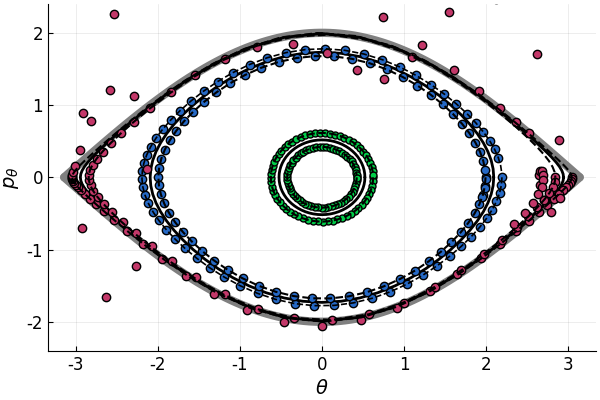
\includegraphics[width=0.7\linewidth]{xi_precision_pendulum}
	\caption{Evaluación del TJ para $\xi = ( \pm 0.1, 0)^T$ en un periodo del péndulo simple en tres distintas secciones para una tolerancia $\epsilon_{Taylor} = 10^{-10}$, jets de orden $M=4$ y expansión de orden $N=24$ Las integraciones nominales de $\xo \pm \xi$ se representan con las curvas negras no sólidas, mientras que la integración para $\xo$ son las curvas negras sólidas. \textit{En verde}: $\xo = (\pi/6, 0)^T$, \textit{En azul}: $\xo = (2\pi/3, 0)^T$ y \textit{En rosa}: $\xo = (15\pi/16, 0)^T$.}
	\label{fig:xi_precision_pendulum}
\end{figure}

Los coeficientes de la expansión de $\flowxi$ dependen de qué tan grandes son las variaciones de las vecindades de la condición tomada para el flujo. La figura \ref{fig:xi_precision_pendulum} muestra cómo para la misma variación $\xi = (\pm 0.1, 0)^T$ el transporte no siempre se comporta de la manera. Más cerca de la separatriz, las evaluaciones se parecen muy poco a flujo real. Así, una forma de controlar qué tan grandes pueden ser las variaciones alrededor de $\xo$ es acotar la contribución del último término a una tolerancia dada; es decir,
\begin{equation*}
 a_{M}^{(n)}\xi_{max}^M \leq \epsilon_{jet}
\end{equation*}
donde $\flowxi = P_{n,\xo}(\xi) = \sum_{|m|=1}^M  a_{m}^{(n)} \xi^m$, con $a_{m}^{(n)}$ el máximo coeficiente $m = \norm{\mathbf{m}}_1$ del jet al tiempo $t_n$.

Se busca controlar el máximo de estos coeficientes, de modo que 
\begin{align}
 \xi_{max} = \min_{|m|=M} \left( \frac{\epsilon_{jet}}{a_{m}^{(n)}} \right)^{\frac{1}{m}}.
 \label{eq:ximax}
\end{align}
es el radio máximo que la vecindad $\Uxo$ puede tomar para estar debajo de la tolerancia impuesta. 

Con ésto se establece qué tan grandes pueden ser las variaciones de $\xo$ sin que las deformaciones del jet repercutan de manera drástica en las soluciones evaluadas. La sección \ref{sec:artificial_ham} muestra cómo la dinámica del campo vectorial exige que las deformaciones de $\Uxo$ sean muy grandes y, como se observó en la figura \ref{fig:artificial_dEjets}, después de cierto tiempo la energía deja de conservarse, lo cual implica que la solución ya no obtenida con el TJ ya no es una buena aproximación de la solución real. Visto de otro ángulo, la vecindad en la que se evaluó era demasiado grande para ser correctamente representada por la parametrización de las soluciones.

%FIGURA!
\begin{figure}[h!]
	\centering
	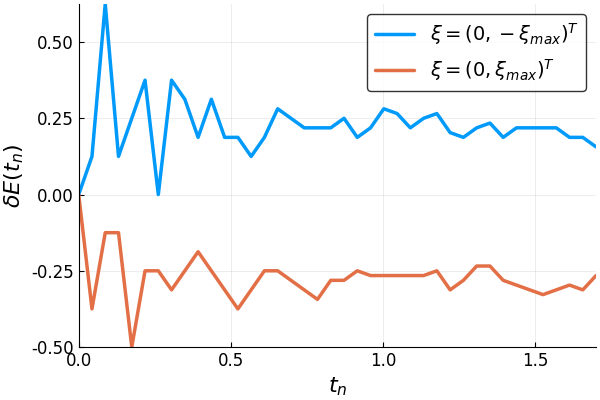
\includegraphics[width=0.7\linewidth]{dE_ximax_ah}
	\caption{Diferencia de energía $\delta E(t_n) = \frac{1}{\epsilon_{machine}} \left( H(\mathbf{x}(t_n)) - H(\xo) \right)$ para el sistema (\ref{eq:artificial_ode}) con jets de orden $M=16$ evaluados en $\xi_{max} = 0.0235$, el cual se calculó con $\epsilon_{jet} = 10^{-14}$. Se utilizó tolerancia $\epsilon_{Taylor} = 10^{-10}$, orden de expansión $N = 25$ y $40$ pasos temporales de $t_0 = 0$ a $t_{max} = 1.7$.}
	\label{fig:dE_ximax_ah}
\end{figure}

En la figura \ref{fig:dE_ximax_ah} retomamos al sistema (\ref{eq:artificial_ode}) que, en su momento, vimos cómo divirgió su energía. Ahora podemos ver que, al establecer una tolerancia $\epsilon_{jet} = 10^{-14}$, las variaciones de energía para ambos casos $\pm \xi_{max}$ son más pequeñas que el épsilon de la máquina. Esto implica que establecer un tamaño máximo de las vecindades reduce drásticamente el error de las soluciones calculadas. Esto, sin embargo, tiene un costo relativamente alto, ya que $\xi_{max} = 0.0235 \ll 0.1$, donde $0.1$ fue la variación respecto a $\xo$ que se había escogido arbitrariamente en la sección \ref{sec:benchmark-taylor}. 

$\xi_{max}$ depende fuertemente de la tolerancia $\epsilon_{jet}$ escogida y, más importante, de la condición inicial en donde se busque saber la variación máxima posible. En general, entre más se deforme el jet con la evolución del flujo, menores serán las vecindades en las que las evaluaciones de $\flowxi$ queden debajo de $\epsilon_{jet}$. Con esto en mente, el tamaño máximo de la vecindad puede servir como un indicador similar a los ELTF, ya que es sensible a la separación entre condiciones iniciales cercanas. El tamaño de vecindad va a detectar grandes gradientes de velocidades, presencia de separatrices en el espacio fase y regiones de caos en órdenes no lineales de la vecindad de las soluciones. Se muestra en la figura \ref{fig:jt_ximax_ah} cómo $\flowU$ consta de una $\Uxo$ considerablemente más pequeña que en \ref{fig:artificial_jt}.

%FIGURA!
\begin{figure}[h!]
 \centering
 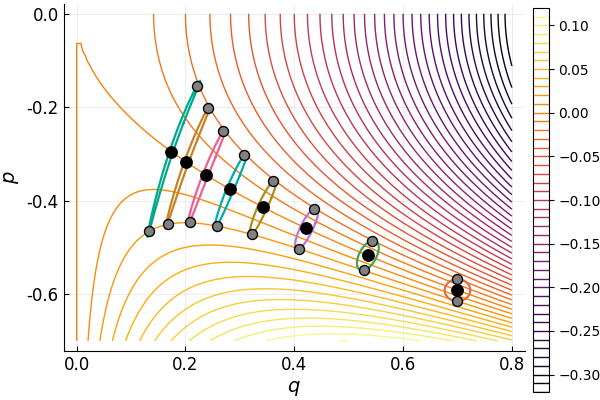
\includegraphics[width=0.7\linewidth]{jt_ximax_ah}
 \caption{Solución para (\ref{eq:artificial_ode}), con condición inicial sobre la separatriz, donde $q_0 = 0.7$. Aquí, los jets son de orden $M=16$, en $8$ pasos de integración desde $t_0 = 0$ hasta $t_{max} = 1.7$, evaluados para $\xi_{max} = 0.025$. Se utilizó tolerancia $\epsilon_{Taylor} = 10^{-20}$ y orden de la expansión $N=25$. En gris están las soluciones a $\xo \pm \xi_{max}$ sin utilizar TJ. La tolerancia para $\xi_{max}$ es de $\epsilon_{jet} = 10^{-5}$.}
 \label{fig:jt_ximax_ah}
\end{figure}

Dicho lo anterior, y a modo de comparar con los ELTF desarrollados previamente, tomemos el caso del péndulo simple, que tiene una separatriz que divide la zona en donde el péndulo oscila respecto a un punto de equilibrio (``rotación'') y la zona donde el péndulo completará periodos completos de oscilación (``libramiento'') . A diferencia de la figura \ref{fig:ftle_pendulum}, la figura \ref{fig:ximax_pendulum} alcanza sus mayores valores en el centro, que es donde las velocidades del campo vectorial son menores y, en cambio, en los valores de la separatriz, se alcanzan los mínimos valores para $\xi_{max}$, ya que es donde los jets sufren mayores deformaciones. Sin embargo, esta figura nos da información equivalente a los ELTF, ya que, cualitativamente, presenta la misma información y nos indica sobre la presencia de la separatriz. De hecho, si las no linealidades de $\xi_{max}$ no contribuyen de manera importante al cálculo de ésta, entonces $\xi_{max}(\xo,T) \propto \frac{1}{\sigma(\xo,T)}$. 

%FIGURA!
\begin{figure}[h!]
 \centering
 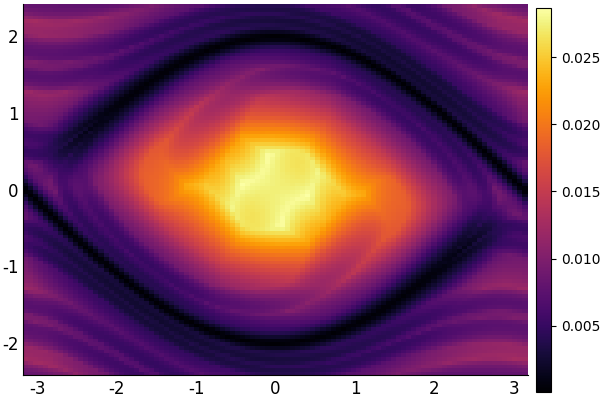
\includegraphics[width=0.7\linewidth]{ximax_pendulum}
 \caption{Campo escalar de los tamaños máximos de vecindad $\xi_{max}$ para el péndulo de (\ref{eq:pendulo-ode}) en una retícula de $60$ puntos por lado, después de un periodo, con tolerancia $\epsilon_{Taylor} = 10^{-10}$ y orden máximo de la expansión $N = 25$.}
 \label{fig:ximax_pendulum}
\end{figure}

%Hacer más ejemplo(s) con esto

\subsection{Tasa de expansión y contracción}
\label{sec:contraccion_expansion}

Otra forma de obtener información sobre los flujos es viendo la tasa de deformación de los jets propagados en el espacio fase. La ventaja de esto sobre el campo escalar de ELTF o del tamaño máximo de vecindades es que aquí es posible saber \textbf{en qué dirección} se tienen la mayor y menor deformación respecto a un punto en el espacio fase. Este indicador se relaciona, en este sentido, con el espectro de Lyapunov, que no es más que el conjunto de eigenvalores $\lambda_i$ obtenidos por las raíces del polinomio característico $P(\lambda) = \det(A - \lambda\mathbf{1})$. El espectro de Lyapunov nos dice cómo crece o se contrae la aproximación lineal de las soluciones bajo un cambio invertible de coordenadas. Las \textbf{tasas de expansión y contracción} de vecindades del flujo $\flowci$ ($\zeta_+$ y $\zeta_-$, respectivamente) nos dicen cuáles son la máxima y mínima separación de $\xo$ con una variación $\xi$ de radio $|\xi(\theta)| = \xi_{max}$.

Para obtener dicho indicador se hace el TJ del orden $M$ deseado integrando hasta $t = t_n$, se obtiene el radio máximo de la vecindad con el método de la sección anterior y se evalúa la frontera de $\Uxo$ en $P_{n,\xo}(\xi(\theta))$. Una vez evaluada, se encuentra el ángulo de máxima (mínima) separación 
\begin{equation}
 \theta_{+}(\xo) = \max_{\theta \in [0,2\pi)} \norm{ P_{n,\xo}(\xi(\theta)) - P_{n,\xo}(0) }
\end{equation} 
y se calcula 
\begin{equation}
 \zeta_{\pm}(\xo) = \frac{ \norm{P_{n,\xo}(\xi(\theta_{\pm})) - P_{n,\xo}(0)} }{\xi_{max}}.
 \label{eq:max_min_rate}
\end{equation}

En el caso de un grado de libertad, como los ejemplos hasta ahora planteados, se ha parametrizado dicha frontera con $\xi(\theta) = \xi_{max} \left( \cos(\theta), \sin(\theta) \right)^T, \theta \in [0,2\pi]$. Evidentemente no se puede evaluar la frontera de $\Uxo$ en un continuo de puntos en la computadora, así que se plantean dos maneras de mejorar la precisión sobre dichos máximos y mínimos: 
\begin{itemize}
\item Aumentar el número de puntos con los cuales se evalúa $\delta \Uxo$
\item Encontrar $\theta_{\pm}$ de los puntos disponibles y luego hacer un Newton-Rapson con $P_{n,\xo}$. 
\end{itemize} 

Se pueden encontrar $\theta_\pm$ y $\zeta_\pm$ para toda una rejilla de puntos y obtener dos campos vectoriales y dos escalares, respectivamente. Los campos vectoriales indican, para cada punto, la dirección de mayor y menor separación de la condición $\xo$ dada; los campos escalares indican la magnitud de esto último. En la figura \ref{fig:seprate_pendulum} se pueden ver ambos campos encimados para el péndulo simple donde, para cada punto de la rejilla, hay un vector en la dirección de máxima (mínima) separación y en color se indica la magnitud de dicha separación.

%FIGURA! 
\begin{figure}[h!]
\centering
\begin{subfigure}{0.49\textwidth}
	\centering
	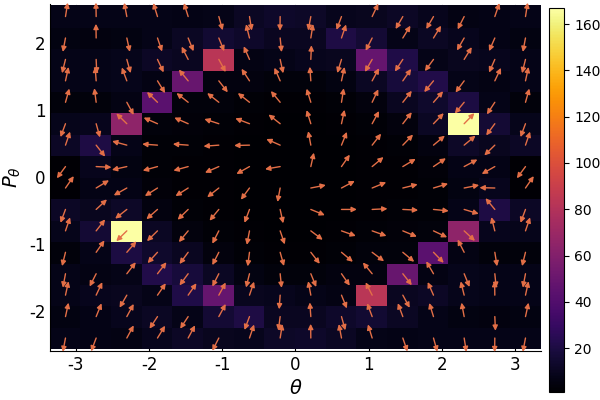
\includegraphics[width = \textwidth]{seprate_max_pendulum}
\end{subfigure}
%
\begin{subfigure}{0.49\textwidth}
	\centering
	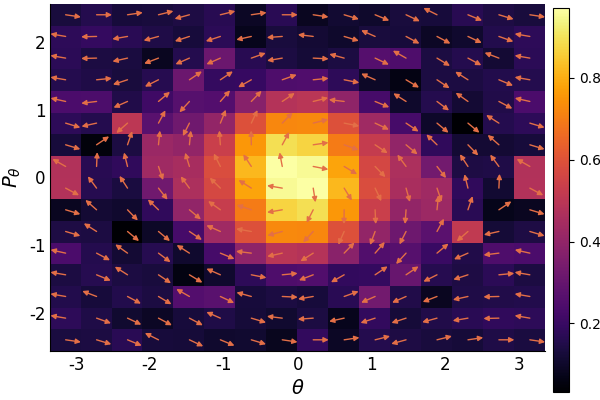
\includegraphics[width = \textwidth]{seprate_min_pendulum}
\end{subfigure}
\caption{ Campos vectoriales dados por $\left( \cos(\theta_\pm(\xo)),\sin(\theta_\pm(\xo)) \right)^T$ sobre los campos escalares $\zeta_\pm(\xo)$ para el péndulo simple, en rejillas de $15\times15$, con tolerancia $\epsilon_{Taylor} = 10^{-20}$, orden de los jets $M=3$ y orden de la expansión $N=25$. \textit{Izquierda}: Campos dados por $\theta_+(\xo)$ y $\zeta_+(\xo)$. \textit{Derecha}: Campos dados por $\theta_-(\xo)$ y $\zeta_-(\xo)$.}
\label{fig:seprate_pendulum}
\end{figure}

Es curioso ver que, para los campos escalares de $\zeta_\pm$, se detecta la presencia de la separatriz en un modo similar que en las dos subsecciones anteriores. De hecho, $\zeta_\pm$ puede utilizarse también como un indicador de separatrices, caos y grandes gradientes de velocidad. La figura \ref{fig:seprate_scalar_pendulum} nos muestra una versión más refinada de los campos escalares correspondientes.\footnote{Se toma la raíz cúbica de $\zeta_\pm$ para achicar la diferencia entre los valores máximos y mínimos y que la imagen sea más legible.} 

%FIGURA!
\begin{figure}[h!]
\centering
\begin{subfigure}{0.49\textwidth}
	\centering
	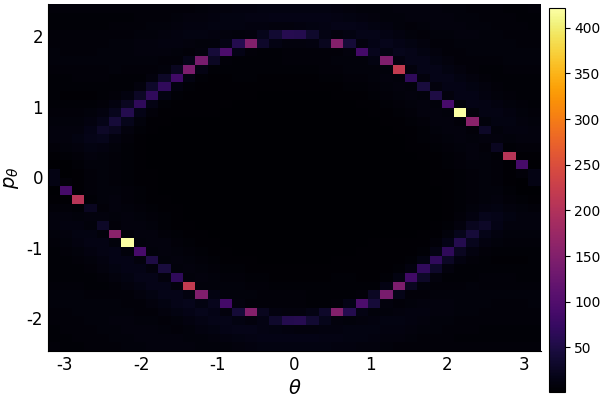
\includegraphics[width = \textwidth]{seprate_max_scalar_pendulum}
\end{subfigure}
%
\begin{subfigure}{0.49\textwidth}
	\centering
	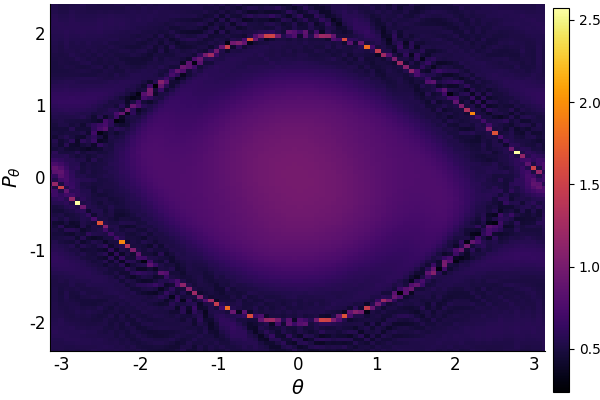
\includegraphics[width = \textwidth]{seprate_min_scalar_pendulum}
\end{subfigure}
\caption{ Campos escalares $\left( \zeta_\pm(\xo) \right)^{1/3}$ para el péndulo simple, en rejillas de $90\times 90$, con tolerancia $\epsilon_{Taylor} = 10^{-20}$, orden de los jets $M=3$ y orden de la expansión $N=25$. Se toma la raíz cúbica para hacer más clara la imagen. \textit{Izquierda}: Campo escalar $\zeta_+(\xo)$. \textit{Derecha}: Campo escalar $\zeta_-(\xo)$.}
\label{fig:seprate_scalar_pendulum}
\end{figure}

%Teniendo xi_max se puede ver en qué dirección se expande más (menos) la deformación de de dx. ESte se hace encontrando el máximo y mínimo en la vecindad evaluada. ¿Cómo serviría esto? 

\subsection{Formas Simplécticas}
\label{sec:formas-simplecticas}
%Motivar un poco porqué hablaríamos de formas simpléticas y decir que el desarrollo viene motivado del chaosbook... si se puede encontrar algún otro libro para complementar estaría muy bien. 

Consideremos la siguiente función
\begin{align*}
H: \mathcal{M} \subset \mathbb{R}^d\times\mathbb{R}^d &\to \mathbb{R} \\ 
	(\mathbf{q},\mathbf{p}) &\to H(\mathbf{q},\mathbf{p})
\end{align*}

que define al hamiltoniano, cuyas ecuaciones de movimiento son

\begin{align*}
 \dot{\mathbf{q}} &= \ \pder{H}{\mathbf{p}} \\
 \dot{\mathbf{p}} &= - \pder{H}{\mathbf{q}}. 
\end{align*}

Si definimos $\mathbf{x} := (\mathbf{q},\mathbf{p}) = (x_1,\ldots,x_{2d})^T$, entonces
\begin{equation}
 \dot{x_i} = \omega_{i,j} \pder{H(\mathbf{x})}{x_j},
 \label{eq:symplectic_ham_ode}
\end{equation}

donde
\begin{equation}
 \omega = 
    \begin{bmatrix}
    \mathbf{0} & \mathbf{I} \\
    -\mathbf{I} & \mathbf{0}
  \end{bmatrix}
 \label{eq:symplectic_omega}
\end{equation}

es una matriz de $2d\times 2d$, $\mathbf{0}$ es una matriz de ceros de $d\times d$ e $\mathbf{I}$ es la matriz identidad de $d\times d$. Notemos que (\ref{eq:symplectic_omega}) cumple
\begin{align}
 \omega^2 &= -\mathbf{I}  \nonumber \\
 \omega^T &= -\omega
 \label{eq:omega_properties}
\end{align}
para cualquier $d$.

\begin{definicion}
Sea $\omega$ una matriz que cumple las propiedades (\ref{eq:omega_properties}). Se dice que una matriz $g$ es \textbf{simpléctica} si
\begin{equation}
 g^T \omega g = \omega.
 \label{eq:symplectic_condition}
\end{equation}
%Ver lo de las formas bilineales... Posiblemente se pueda partir de una definición más formal/general y concluir esto para g. 
\end{definicion}

Las matrices que cumplen la definición anterior forman un \textbf{grupo simpléctico} denotado $Sd(d)$, que son un caso particular de los grupos de Lie.

Los \textbf{grupos de Lie} son grupos cuyos elementos dependen de un número finito de parámetros, i.e., $g = g(\eta) = g(\eta_1,\ldots,\eta_N)$. Dicho esto, y como se menciona en \cite{CBHamiltonianDynamics}, para los cálculos se suele escoger una base para operar dichas matrices y, para transformaciones infinitesimales del espacio fase, éstas toman la forma
\begin{equation}
 g(\delta \eta) := \mathbf{1} + \delta \eta \mathbf{T},
 \label{eq:symp_infinit_rotation}
\end{equation}

con $\lbrace T_1, \ldots, T_N \rbrace$ un conjunto de rotaciones\footnote{Dichas rotaciones representan las deformaciones infinitesimales de las transformaciones de $g$.} sobre el espacio fase.

Notemos que si al grupo de rotaciones (\ref{eq:symp_infinit_rotation}) le imponemos la condición (\ref{eq:symplectic_condition}) de simplecticidad

\begin{align*}
  \left( \mathbf{1} + \delta \eta \mathbf{T} \right)^T \omega \left( \mathbf{1} + \delta \eta \mathbf{T} \right) = \omega \implies 
  \cancel{\omega} + (\delta \eta \mathbf{T})^T \omega + \omega \delta \eta \mathbf{T} + \cancelto{\mathcal{O}(\norm{\delta \eta \mathbf{T}}^2)} {(\delta \eta \mathbf{T})^T \omega \delta \eta \mathbf{T}} = \cancel{\omega}, 
\end{align*}

obtenemos una forma explícita para que éste sea simpléctico
\begin{equation}
  (\delta \eta \mathbf{T})^T \omega + \omega \delta \eta \mathbf{T} = \mathbf{0}.
  \label{eq:eq:symplectic_condition2}
\end{equation}

En el caso de tener un hamiltoniano $H(\mathbf{x})$, basta darse cuenta que
\begin{itemize}
\item $H(\mathbf{x})$ es, al menos, $\mathcal{C}^2(\mathcal{M})$; esto es, $\frac{\partial^2 H}{\partial x_i \partial x_j} = \frac{\partial^2 H}{\partial x_j \partial x_i}$.

\item Los generadores de las transformaciones infinitesimales del sistema de EDO (\ref{eq:ode}) están dadas por $A_{i,j}(\mathbf{x}) := \pder{f_i(\mathbf{x})}{x_j}$. $A_{i,j}(\mathbf{x})$ son los elementos de matriz de $A(\mathbf{x})$, la cual se conoce como \textbf{matriz de estabilidad} del sistema.

\item La matriz de estabilidad puede representarse en términos de $\omega$ como $A(\mathbf{x}) = \omega \Xi(\mathbf{x})$, donde $\Xi(\mathbf{x}) = \left[ \frac{\partial^2 H(\mathbf{x})}{\partial x_i \partial x_j} \right]$ es el \textbf{hessiano}, o matriz de segundas derivadas, de $H$.

\item Como $H$ es $\mathcal{C}^2(\mathcal{M})$, entonces $\Xi$ es simétrica y, por tanto, $\Xi = \Xi^T$.
\end{itemize}

Con las observaciones anteriores podemos ver que
\begin{align*}
 A(\mathbf{x})^T \omega + \omega A(\mathbf{x}) = \Xi(\mathbf{x})^T \cancelto{\mathbf{I}}{\omega^T \omega} + \cancelto{-\mathbf{I}}{\omega \omega}\Xi(\mathbf{x}) = \Xi(\mathbf{x})^T - \Xi(\mathbf{x}) = 0.
\end{align*}

Así, cualquier sistema hamiltoniano es un sistema simpléctico y cumple
\begin{equation}
 A^T\omega + \omega A = 0
 \label{eq:symplectic_hamiltonian}
\end{equation}
%Meterlo como corolario o teorema? Chance es más elegante.

%Valdrá la pena hablar/demostrar que la simplecticidad implica la conservación de volumen? 

Regresemos, como siempre, al caso del péndulo simple. Sabemos, por (\ref{eq:pendulo-ham}), que es un sistema hamiltoniano y, por tanto, debe de cumplir (\ref{eq:symplectic_hamiltonian}). La matriz de estabilidad de éste\footnote{Se toma, sin pérdida de generalidad, $g = m = l = 1$.} está dada por
\begin{equation*}
  A_{pend}(\theta,p_\theta) =
  \begin{bmatrix}
    0             & 1 \\
    -\cos(\theta) & 0
  \end{bmatrix},
\end{equation*}

entonces

\begin{align*}
  A_{pend}^T \omega + \omega A_{pend} &=
  \begin{bmatrix}
    0 & -\cos(\theta) \\
    1 & 0
  \end{bmatrix}   
  \begin{bmatrix}
    0  & 1 \\
    -1 & 0
  \end{bmatrix} 
  +
  \begin{bmatrix}
    0  & 1 \\
    -1 & 0
  \end{bmatrix} 
  \begin{bmatrix}
    0             & 1 \\
    -\cos(\theta) & 0
  \end{bmatrix} \\
  &=
  \begin{bmatrix}
    \cos(\theta)  & 0 \\
    0             & 1
  \end{bmatrix}
  +
  \begin{bmatrix}
    -\cos(\theta)  & 0 \\
    0              & -1
  \end{bmatrix}
  = 0 
\end{align*}

probando ``a mano'', que es un sistema simpléctico. Sin embargo, la matriz de estabilidad también se calculó a mano, y ese es un proceso que la construcción polinomial del Transporte de Jets nos puede ahorrar. Dado que parametrizamos las vecindades de la condición inicial vía $\xo \to \xo + \xi = P_{0,\xo}(\xi)$, si evaluamos $P_{0,\xo}(\xi)$ en el campo vectorial $f$ obtendremos la parametrización de éste alrededor de $\xo$ y, como la evaluación es un vector de polinomios en $\xi$, se puede obtener la matriz de estabilidad, cuyos elementos son $A_{i,j}(\xi) = \pder{f_i(P_{0,\xo=(0,0)}(\xi))}{\xi_j}$.

Ahora, el problema de probar la simplecticidad de esta manera es que la expansión $P_{0,(0,0)}(\xi)$ es una expansión finita y no representa necesariamente a $f(\xi)$. Sin embargo, resulta ser que si un sistema es hamiltoniano, el correspondiente sistema dado por la expansión de sus funciones en series de Taylor hasta orden $M < \infty$ también lo es.

\begin{teorema}
Sea 
\begin{align*}
  H: \mathcal{M} \subset \mathbb{R} \times\mathbb{R} &\to \mathbb{R} \\ 
  (q,p) &\to H(q,p)
\end{align*}
una función escalar que define al sistema
\begin{align}
 \dot{q} &= \ \pder{H}{p} = f_1(q,p) \nonumber \\
 \dot{p} &= - \pder{H}{q} = f_2(q,p).
 \label{eq:theorem_ode}
\end{align}
Si $f_i$ es $\mathcal{C}^\omega(\mathcal{M}) \ \forall i$, entonces $\exists! \  \mathcal{H}: \mathcal{M} \to \mathbb{R}$ que define a
\begin{align*}
 \dot{q} &= \ \pder{\mathcal{H}}{p} = P_{f_1}^M(q,p) \\
 \dot{p} &= - \pder{\mathcal{H}}{q} = P_{f_2}^M(q,p)
\end{align*}
con $P_{f_i}^M(q,p)$ el desarrollo de Taylor de orden $M$ de $f_i$.
\footnote{El teorema es generalizable para $\mathcal{M} \subset \mathbb{R}^d \times \mathbb{R}^d$. La demostración queda como ejercicio para el lector.}
\end{teorema}

\begin{proof}
Como $f_i$ es $\mathcal{C}^\omega(\mathcal{M}) \ \forall i$, pueden expresarse como
\begin{align*}
 f_1(q,p) &= \sum_{i,j = 0}^\infty a_{i,j} q^i p^j \\
 f_2(q,p) &= \sum_{i,j = 0}^\infty b_{i,j} q^i p^j. 
\end{align*}
Así, por (\ref{eq:theorem_ode}), resolvemos $H(q,p)$ integrando
\begin{align*}
 H(q,p) &= \int f_1(q,p) dp = \sum_{i,j = 0}^\infty \frac{a_{i,j}}{j+1} q^i p^{j+1} + \ell_1(q) \\
 H(q,p) &= -\int f_2(q,p) dq = -\sum_{i,j = 0}^\infty \frac{b_{i,j}}{i+1} q^{i+1} p^j + \ell_2(p)
\end{align*}
encontrando la relación 
\begin{equation*}
 \frac{a_{i+1,j}}{j+1} = - \frac{b_{i,j+1}}{i+1} 
\end{equation*}
y la forma explícita de $\ell_i$
\begin{align*}
 \ell_1(q) &= \sum_{i=0}^\infty \frac{b_{i,0}}{i+1} q^i \\
 \ell_2(p) &= \sum_{i=0}^\infty -\frac{a_{0,i}}{i+1} p^i.
\end{align*}
Como todo lo anterior es cierto término a término, podemos truncar a cualquier orden $M < \infty$ y construir $\mathcal{H}$ con las expansiones truncas $P_{f_1}^M(q,p)$ y $P_{f_2}^M(q,p)$. \qed
\end{proof}

\begin{corolario}
Si $H$ define un sistema hamiltoniano, entonces $\mathcal{H}$ es simpléctico. 
\end{corolario}

Así, como sabemos que los ejemplos construidos hasta ahora vienen de un hamiltoniano $H(q,p)$, entonces la expansión polinomial $f(P_{0,(0,0)}(\xi))$ define una matriz de estabilidad simpléctica. 

Otra forma de ver la simplecticidad de un sistema es usando directamente (\ref{eq:symplectic_condition}) e interpretando la matriz $g$. Hay una visión geométrica que plantea Arnold \cite{Arnold1989} en su capítulo de variedades simplécticas, donde una estructura simplética es una 2-forma cerrada, lo cual representa la conservación del espacio fase. De este modo, la matriz $g$ se puede representar con el jacobiano de $\phi(t;t_0,\xo)$ y, para cualquier tiempo $t$ del flujo, un sistema es simpléctico cumple
\begin{equation}
 J(\phi(t))^T \omega J(\phi(t)) = \omega \ \forall t.
 \label{eq:sympletic_flow}
\end{equation} 
tal como se propone en la sección 42 de dicho capítulo del Arnold.

Esta forma de ver la simplecticidad es una mejor opción para ver qué tan buena es la integración de un sistema Hamiltoniano dado. Como el Transporte de Jets parametriza las vecindades de una trayectoria en el espacio fase, se puede obtener fácilmente el jacobinano para cada punto de ésta, y comprobar la simplecticidad de los sistemas se vuelve un proceso bastante directo una vez obtenida la solución. En este sentido, además de cualquier constante de movimiento que pueda tener un sistema, éste es un indicador de qué tan buena es la integración siempre que se tenga un sistema hamiltoniano.

%FIGURA! 
\begin{figure}[h!]
 \centering
 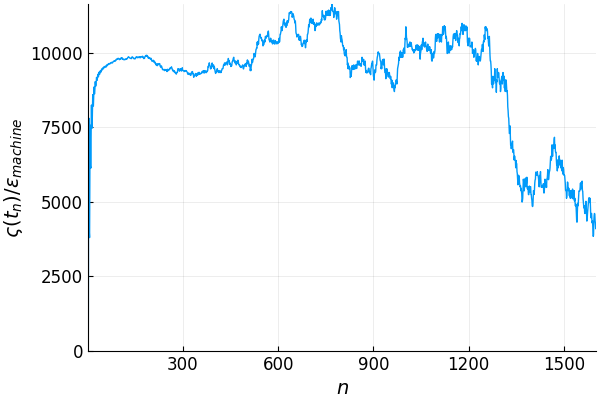
\includegraphics[width=0.8\linewidth]{simplecticity_pendulum}
 \caption{Representación escalar de la simplecticidad del péndulo simple con condición inicial $( \pi/2,0)^T$ para $200$ periodos ($1600 $ pasos de integración) con orden del jet $M=2$, orden de la expansión $N = 28$ y tolerancia $\epsilon_{Taylor} = 10^{-10}$.}
 \label{fig:simplecticity_pendulum}
\end{figure}

La figura \ref{fig:simplecticity_pendulum} muestra la variación de la cantidad $\varsigma(t)$ para el péndulo simple en términos de $\epsilon_{machine}$. Ésta se define como
\begin{equation}
 \varsigma(t) = \norm{ J(\phi(t))^T \omega J(\phi(t)) - \omega }_\infty
 \label{eq:scalar_symplecticity}
\end{equation}
y no es más que el máximo valor absolutos de la matriz de (\ref{eq:sympletic_flow}). $\varsigma$ es una forma escalar de representar la simplecticidad del sistema para poder visualizarlo gráficamente para cada paso temporal.
  
Podemos observar en dicha figura un comportamiento browniano, similar a como pasa con la energía en los ejemplos de sistemas hamiltonianos planteados hasta ahora.


\subsection{Parametrización de parámetros}
\label{sec:parameter_variation}
Aunque el título de esta sección suene redundante, el TJ nos permite no sólo parametrizar las vecindades de $\xo$ en un campo vectorial dado sino también los parámetros que lo definen.

Tomemos, por ejemplo, al oscilador armónico dado por  
\begin{equation}
 \ddot{x}(t) + \omega^2 x(t) = 0,
 \label{eq:one_dim_oscil}
\end{equation}

con hamiltoniano
\begin{equation}
 H(x,y) = \frac{1}{2} \left( y^2 + \omega ^2 x^2 \right),
 \label{eq:osc_ham2}
\end{equation}
con $y = \dot{x}$ y $\omega \in \mathbb{C}$.

Complejificando el dominio, sabemos la solución
\begin{equation*}
 x_{\mathbb{C}}(t) = A e^{i\omega t} + B e^{-i \omega t},
\end{equation*}
donde, si $\omega^2 > 0$, entonces la proyección a los reales es
\begin{equation}
 x(t) = a \cos(t) + b \sin (t)
 \label{eq:ho_solution_trig}
\end{equation}
y, si $\omega^2 < 0$, la proyección es
\begin{equation}
 x(t) = \alpha e^{\omega t} + \beta e^{- \omega t}.
 \label{eq:ho_solution_exp}
\end{equation}

%FIGURA!
\begin{figure}[h!]
 \centering
 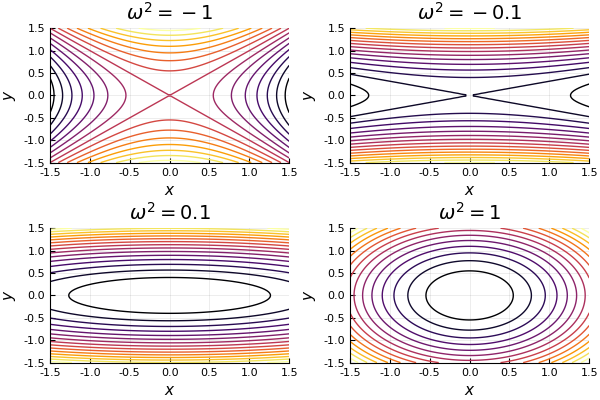
\includegraphics[width=0.8\linewidth]{oscillator_domega}
 \caption{Curvas de nivel dadas por (\ref{eq:osc_ham2}) para diferentes valores de $\omega^2$.}
 \label{fig:oscillator_domega}
\end{figure}

Observamos en la figura \ref{fig:oscillator_domega} cómo las curvas de nivel cambian para distintas $\omega^2$; en particular, observamos que las soluciones cambian de topología cuando $\omega^2$ cambia de signo. Con esto, pensar en una \textit{parametrización del parámetro} resulta una herramienta poderosa en el estudio de este tipo de sistemas ya que, por un lado, puede funcionar como un indicador para cambios de topología o bifurcaciones de las soluciones y, por otro, ayudar a encontrar conjuntos de soluciones cuando los parámetros no se conocen con exactitud. 

Para hacer esto con el Transporte de Jets, basta con incluir al parámetro o los parámetros que se quieran variar en el sistema de ecuaciones como $\dot{\lambda} = 0$, donde $\lambda$ es el conjunto de parámetros que se quieren variar. En este ejemplo el sistema queda como
\begin{align*}
 \dot{x} &= y \\
 \dot{y} &= - \omega^2 x \\
 \dot{\omega^2} &= 0.
\end{align*}
 
%FIGURA! 
\begin{figure}[h!]
 \centering 
 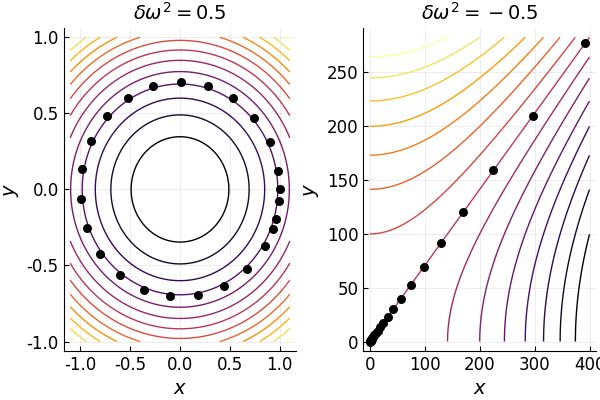
\includegraphics[width=0.8\linewidth]{oscillator_domega2}
 \caption{Solución para condición inicial $\xo = (1,0,0)$ y variación del parámetro para $\delta \omega^2 = 0.5$ en la izquierda y $-0.5$ en la derecha. $\delta \omega$ es un polinomio de orden $30$, y el desarrollo de Taylor para la solución es de orden $28$, con tolerancia de $10^{-20}$. Son $25$ pasos de integración de $0$ a $2 \pi$.}
 \label{fig:oscillator_param_transport}
\end{figure}

La figura \ref{fig:oscillator_param_transport} muestra el trasnporte de jets para $\omega^2$ para la condición inicial $\omega^2 = \omega_0^2 + \delta \xi$. En este caso $\omega_0^2 = 0$ y $\delta\xi = \pm 0.5$. Resulta que el Transporte de Jets sí muestra el cambio de topología dado por el signo de $\omega^2$. Sin embargo, hay que ver qué tan precisa es la solución, lo cual se puede checar con la conservación de la energía al evaluar el hamiltoniano. 

El flujo conserva la energía cada vez menos conforme pasa el tiempo como se observa en la figura \ref{fig:oscillator_dE_domega}; de hecho, la solución que diverge más pierde hasta $15000$ epsilons casi al final de la integración. Sin embargo, el error máximo en términos absolutos es de $3.63 \times 10^{-12}$, lo cual es bastante aceptable.

%FIGURA! 
\begin{figure}[h!]
 \centering
 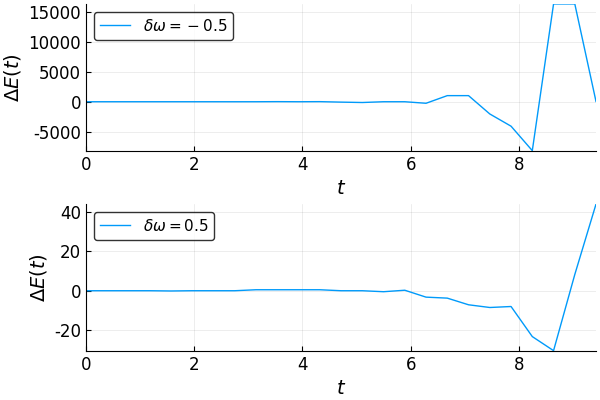
\includegraphics[width=0.8\linewidth]{oscillator_dE_domega}
 \caption{Variación $\Delta E = \frac{1}{\epsilon_{machine}} \left( E(t) - E_0 \right)$ de la energía respecto a la condición inicial para ambas evaluaciones del transporte $\delta \omega < 0$ y $\delta \omega > 0$.}
 \label{fig:oscillator_dE_domega}
\end{figure}


Los indicadores desarrollados hasta ahora refuerzan el estudio del espacio fase como en los campos escalares y vectoriales de $\xi_{max}$ y $\theta_{\pm}$, permiten tener alternativas al método de Montecarlo como en la parametrización de parámetros, nos dan formas de evaluar las vecindades en un radio donde el error sea menor a una tolerancia dada y permiten corrobrar la simplecticidad de un flujo hamiltoniano. Éstas se utilizarán en un problema específico, el \textbf{problema circular de tres cuerpos}, el cual se desarrollará en el siguiente capítulo.
%Pequeña conclusión de sección ? 